\documentclass[dvipdfmx]{jsarticle}
\usepackage{amsmath,amssymb}
%¥usepackage{mathpazo}
\usepackage{amsthm}
\newtheorem{dfn}{定義}
\newtheorem{thm}[dfn]{定理}
\newtheorem{lem}[dfn]{補題}
%\usepackage{newtxtext,newtxmath}
%\usepackage[hiresbb]{graphicx}
%¥図
\usepackage{bm}
%¥ボールド体
%\usepackage{mathrsfs}%ラグラジアン
\usepackage{wrapfig}%¥図の周りに文章を回り込ませる
\usepackage[dvipdfmx]{graphicx,color}
\usepackage{pgfplots}
\pgfplotsset{compat=1.16}
\usetikzlibrary{intersections,calc,arrows.meta,decorations.pathmorphing,backgrounds,positioning,fit,petri}
\usepackage{array}
\usepackage{siunitx}
\usepackage[version=3]{mhchem}
\usepackage{float}
\newcommand{\setN}{\mathbb{N}}
\newcommand{\setZ}{\mathbb{Z}}
\newcommand{\setQ}{\mathbb{Q}}
\newcommand{\setR}{\mathbb{R}}
\newcommand{\setC}{\mathbb{C}}
\usepackage{physics}
\usepackage{tcolorbox}
\usepackage[dvipdfmx]{hyperref}
\usepackage{pxjahyper}
\usepackage{tikz}
%\usepackage{gnuplot-lua-tikz}
\usepackage{subfigure}
\hypersetup{colorlinks=true}
\makeatletter
\@addtoreset{equation}{section}
\def\theequation{\thesection.\arabic{equation}}
\makeatother
\title{物性物理学第三} 
\author{Eymmetry \thanks{\url{https://twitter.com/Eymmetry}}}
\date{\today}
\begin{document}
\maketitle
\section{紹介}
ここではガイダンスを行う。
まずは光物性から
すべてを量子力学から扱って説明するのが最終的な求められる記述であるが底までやらなくても現象を十分説明できるのが今の認識である。
電場に関する応答を
\[
\bm{D}=\varepsilon \bm{E}
.\] 
誘電率は一般にテンソル量である。
これを拡張して
\[
\bm{D}(\omega)=\varepsilon(\omega)\bm{E}(\omega)
.\] 
このとき$\omega$ に依存する誘電率を応答関数という。
この誘電関数というものを
便宜的に複素数で考える。
\[
\varepsilon(\omega)=\varepsilon'(\omega)+i\varepsilon''(\omega)
.\] 
これは屈折率から図れる。
応答をふくそすうであらわすわけであるがこれは便宜的なものである。

電場を周期的に与えたときに位相の遅れをふくそすうのぶぶんでかん替えているだけ。
量子力学だと物理量そのものが複素数ということもあるがここではそいういうことではない。

この誘電関数というものをもとめていくのが基本的な問題になる。

金属と絶縁体に分けて考えてみる。
絶縁体というのはバンドギャップがあって光を当てると電子が励起される。
これを古典的なモデルであるローレンツモデルで考える。

電場を当てるとバネが伸び縮して反応する。これを共振が起こる。
電子双極子の集まりとして考えて応答を観測する。

金属の場合には全く異なり伝導電子を持っていてこれによって電場を加えたときに遮蔽という現象が起こる。
こうすると誘電率というのが静的に定義できない。
振動数が高くなってくると振動が追いつかなくなるということが起こる、この途中のプラズマ振動数で何かが起こる。これより高い周波数で勤続中に電磁波が伝搬する。

このプラズマ振動数は可視光と紫外線の間くらいになる。

これによって金属の色とかわかってくる。
\begin{figure}[H]
	\centering
	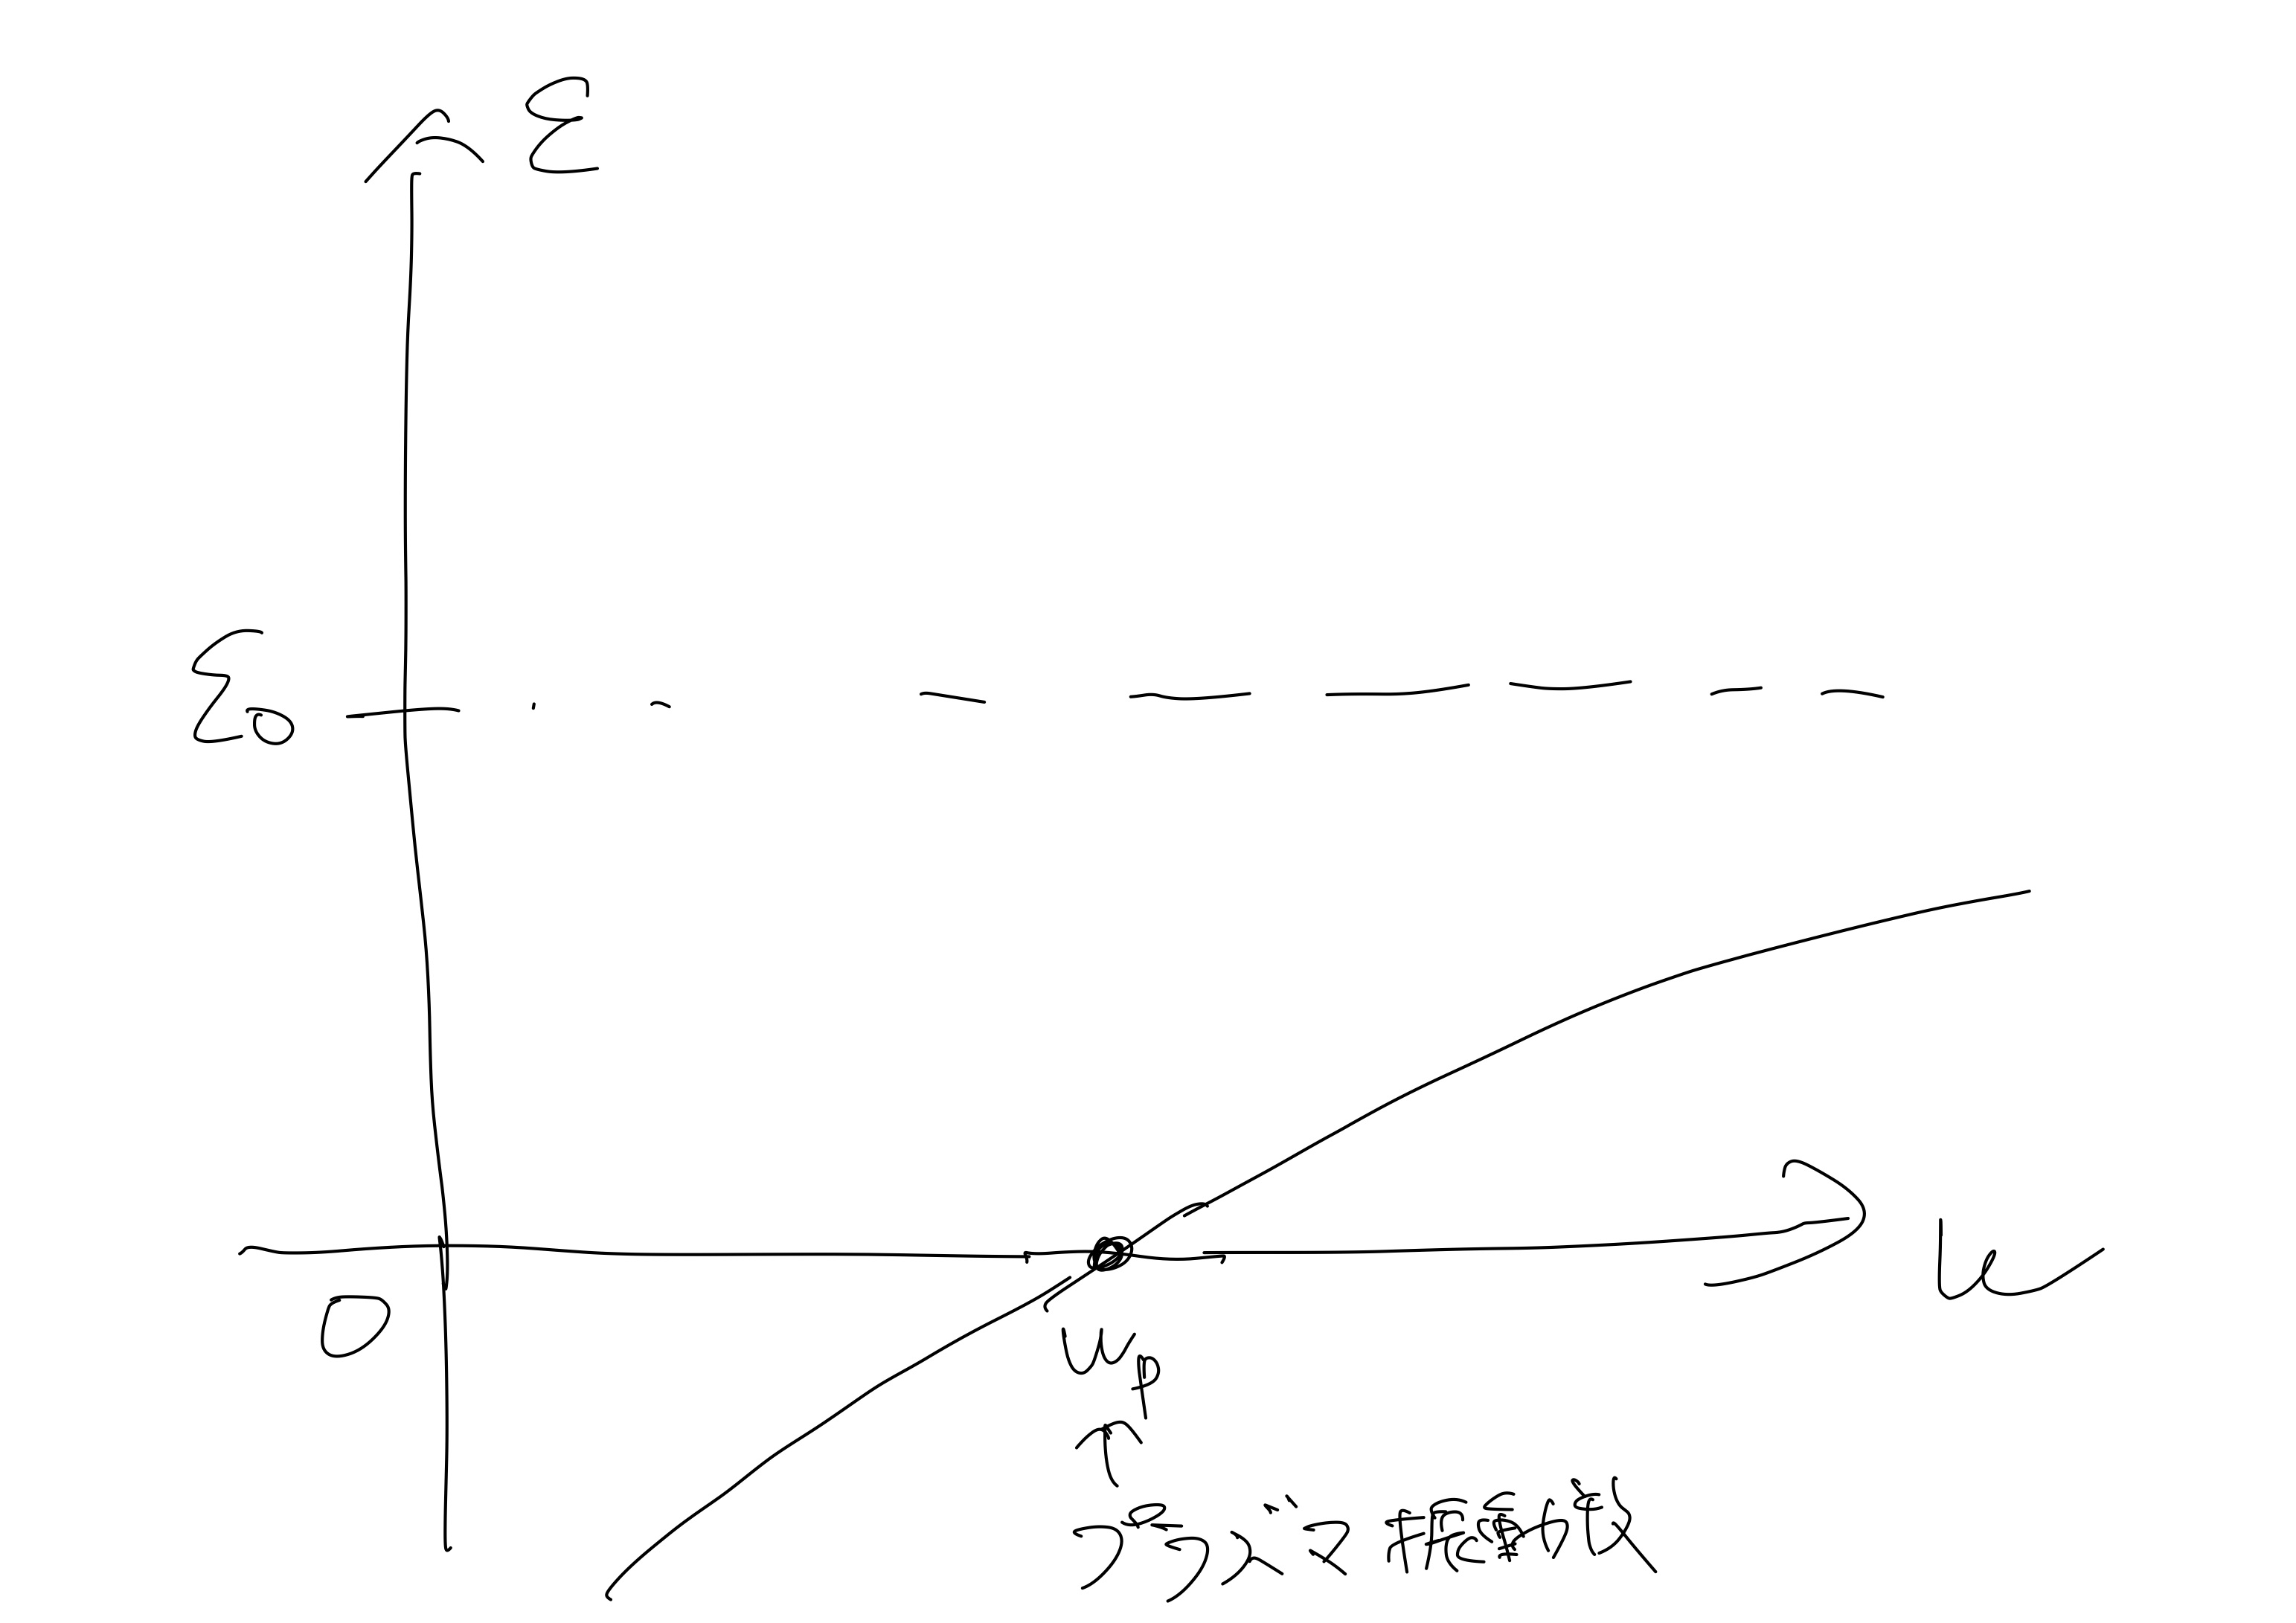
\includegraphics[width=0.5\textwidth]{fig1/Fig-3.jpg}
	\caption{fig1/Fig-3.jpg}
	\label{fig:fig1-Fig-3-jpg}
\end{figure}

つづいて磁性について
まず磁性という性質は古典的には説明できない。
この磁気モーメントの発生する原因がスピン角運動量でありこれは古典的には説明できない。
古典的なモデルでは磁気モーメントがなくなるということがわかる( なんかそういう定理があるはず)。
磁性はほとんどの物質ではでない。普通磁石になるような物質というのは希土類と遷移金属が含まれている。これ以外の物質で磁石になるやつは今までにない。

\[
H=-\sum_{<i,j>}^{}J_{ij} \bm{S}_i\cdot \bm{S}_j
.\] 
$J_{ij}$ を正確に計算するというのは難しい。
波動関数の重なりに起因する相互作用であり、隣り合ったところからちょっとでも離れると考えなくて良くなるので隣り合った奴らだけ考える。
こうやって考えたときに$J<0,>0$ の場合がある。
これによって強磁性か反強磁性かがきまる。
これを簡単に考えるために分子場理論とか平均場理論とかを考えていく。
これは周りからの相互作用を自己無同着な形で方程式を解いていくことによって磁化とかを出していく。

また伝導電子が示す磁性というものありこれはパウリ譲二性とかランダウ判事性がある。これは電子がスピン、ランダウ判事性は電子の輝度運動からでるものである。
これは理論亭な取扱はすが置く難しいがまだちゃんとわかっていない。
例えば鉄とかニッケルが磁石になるのは格子点に止まっているきょくざいしたやつが磁石になるだけでは説明できなくてこれを伝導電子にも拡張するのはわかっていない。これを現象論的に認めて議論を進めていく。


最後に超電導の基本的な事柄について熱力学と統計力学で考える。
\begin{figure}[H]
	\centering
	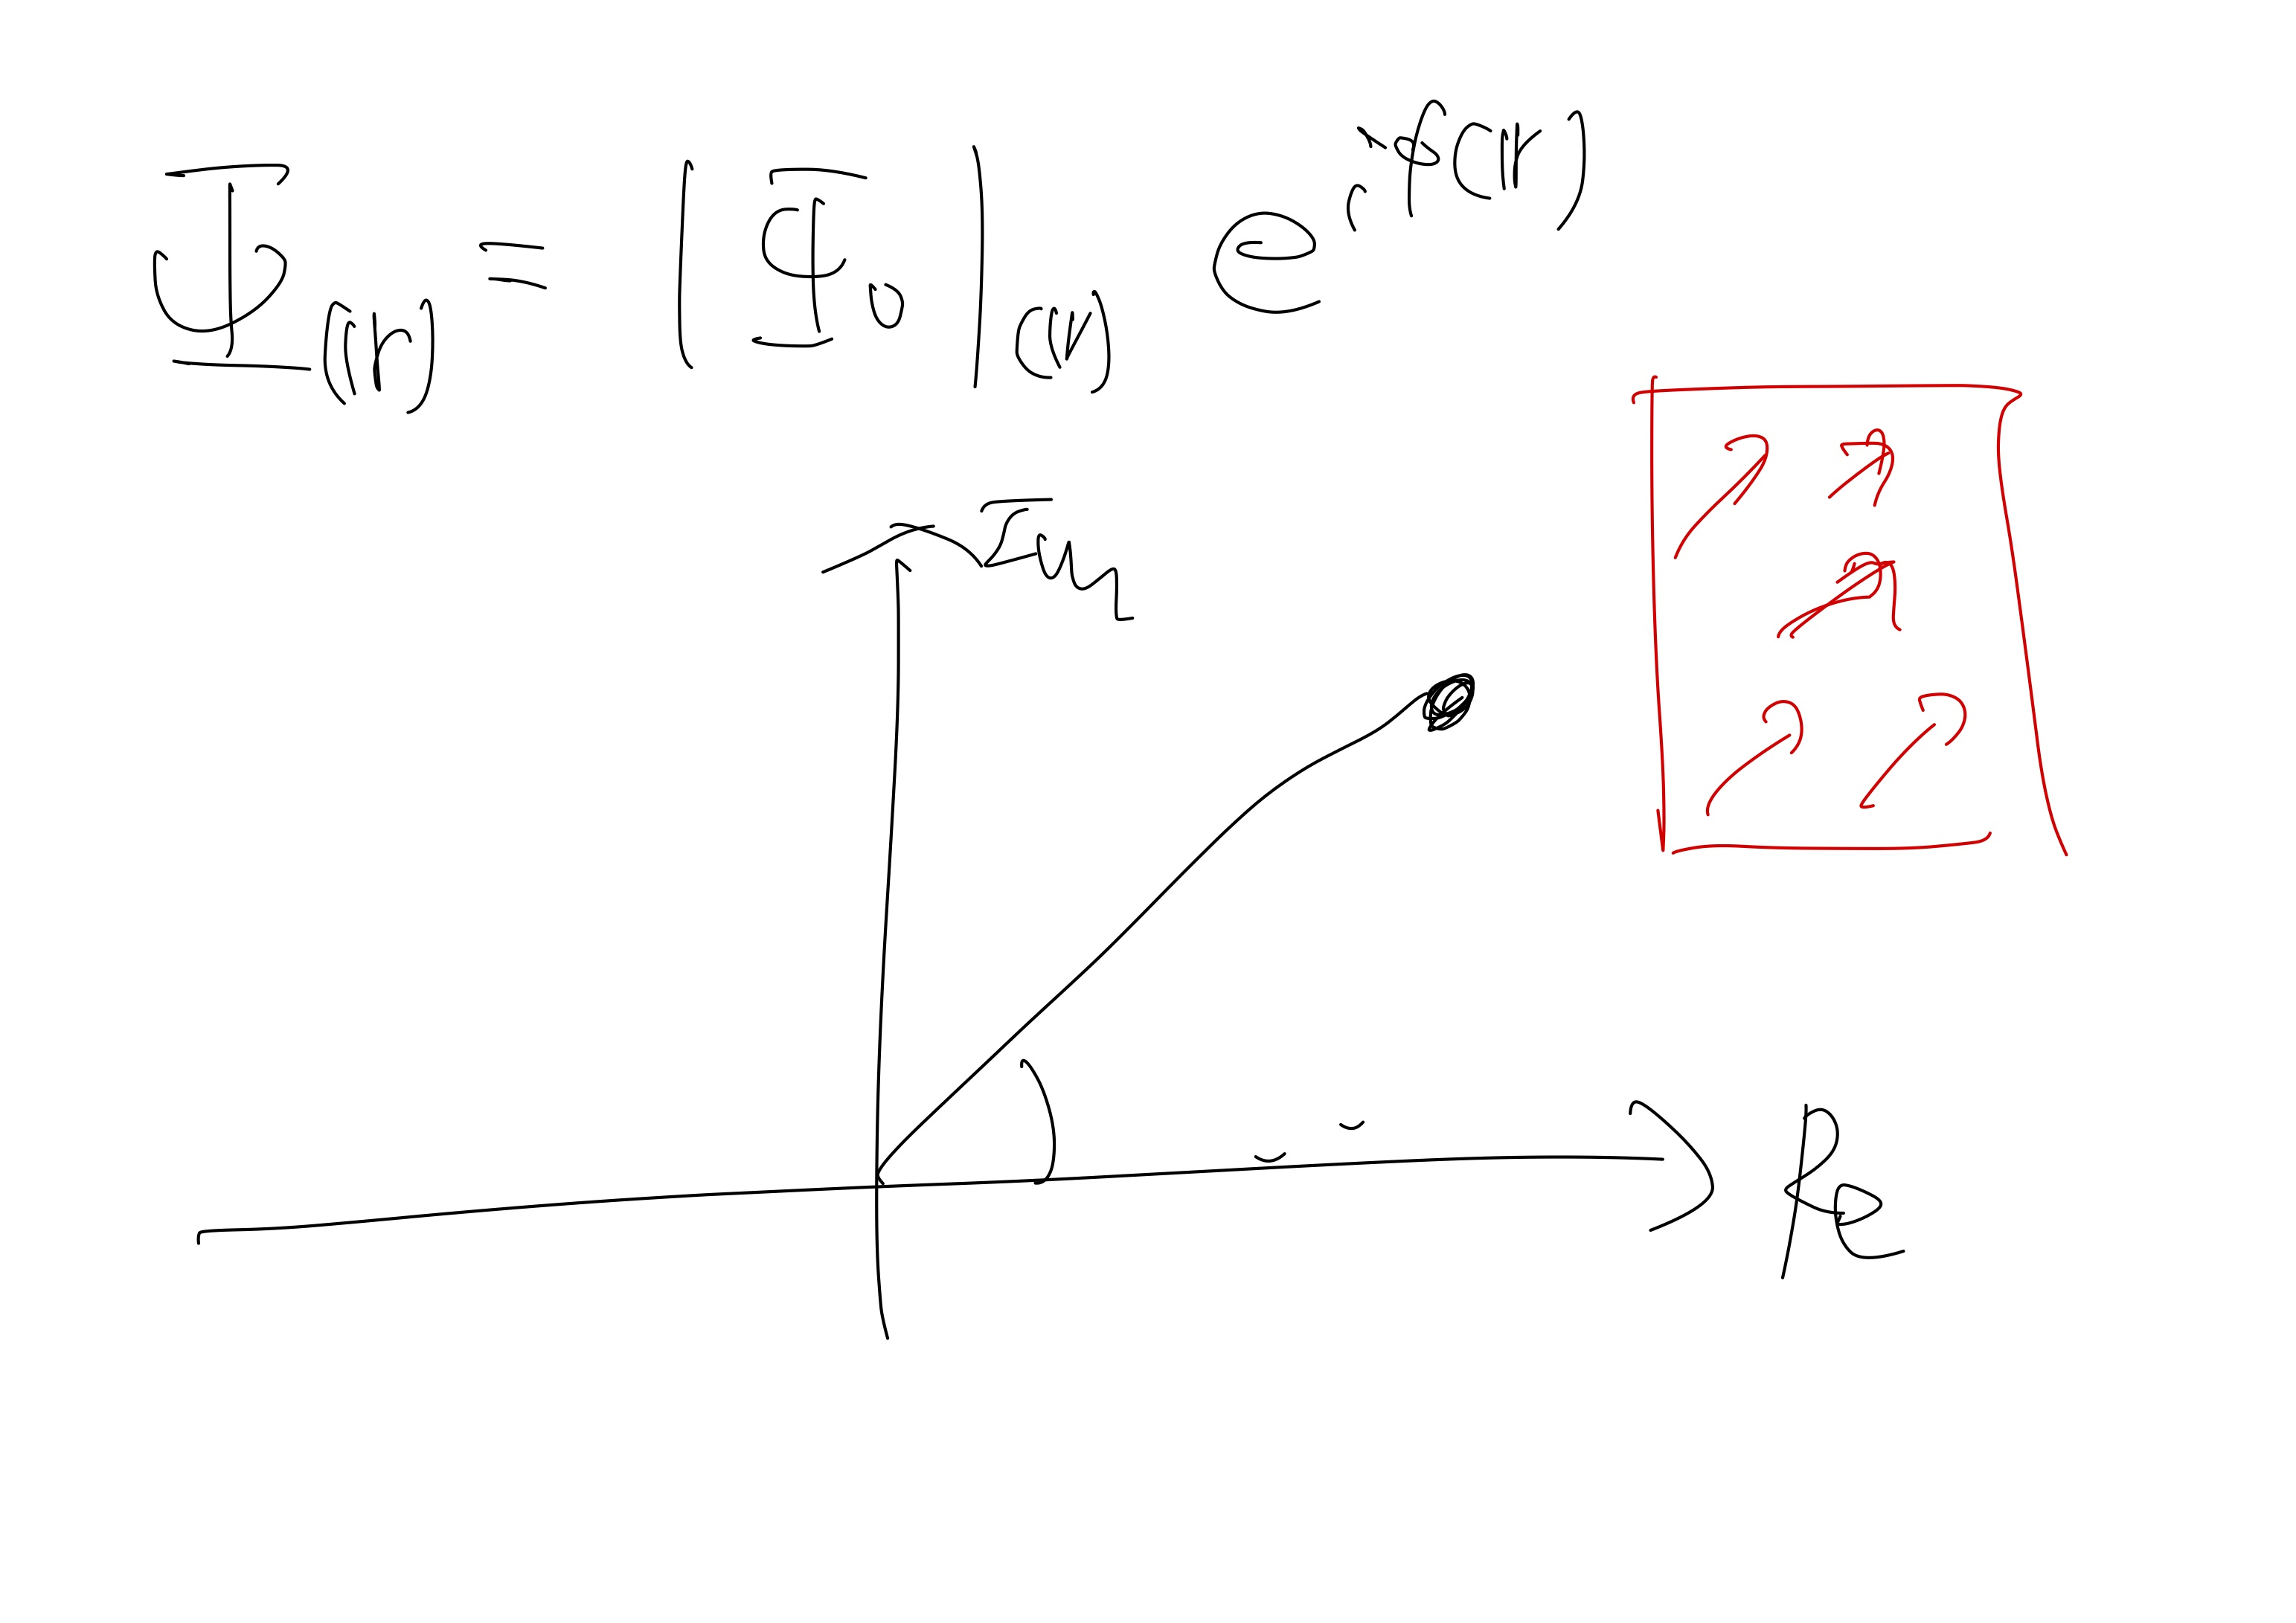
\includegraphics[width=0.5\textwidth]{fig1/Fig-4.jpg}
	\caption{fig1/Fig-4.jpg}
	\label{fig:fig1-Fig-4-jpg}
\end{figure}
ちょうでんどうがある秩序を持ったものとして考えて秩序パラメータを導入する。これは複素数である。
例えば磁性において臨海温度よりも低温ではスピンが同じ方向を向いている。このときにこれを巨視的な一つの磁化とかんがえると、これは時期秩序を表すへんすうになっていて秩序変数とか秩序パラメ多という。
そうすると磁化がゼロでないときとゼロのときという状態が考えられて,

超伝導体の中には複素空間があってバラバラな向きを向いて賞味ゼロだったのが超伝導になるとこの矢印が揃ってしまうということがわかる。

磁性体の中でもXY模型と超電導はと等価である。

ここだけではまだ不十分でBCS理論がなきゃだめ。これは電子がフェルミ球を作っている不安定になると原子は束縛状態をとったほうが安定する。つまり対を作ろうとする。これがBCS理論。

あとは授業で扱わないやるもあるが、強相関とかトポロジカル物質とかは扱わない。近藤効果も扱わない。
\end{document}
